\section{Testing}
\subsection{Environments}
For testing our encodings we decided on what instances to test on beforehand. We specified three domains with instances with increasing malfunction density (probability of malfunctions).

The \textbf{sparse} domain (Figure \ref{sparse_0_1_fullpage}) consists of $60\times60$ maps with 6 cities and 6 trains. The original goal, was to do a 100x100 map with 3 trains. But that would simplify the pathfinding and malfunction handling too much, to properly see how the encodings perform. The 6 cities were a necessity as Flatland on a 60x60 map with two cities, often generated maps, which only use a small section of the map, being more akin to a $30\times30$ map. The interest of this map is mainly to check our graph representation and how it performs with big maps (also requiring many timesteps).

The \textbf{dense} domain (Figure \ref{dense_0_1_fullpage}) consists of 24x24 maps with 3 cities and 20 trains. This is the smallest possible dimension for generation and mainly focuses on malfunction handling. More trains, lead to more malfunctions and require efficient ways of handling them.

The \textbf{medium} domain (Figure \ref{medium_0_1_fullpage}) is a middle ground, of $50\times50$, 5 cities and 10 trains.

To ensure comparability, all domains above specify that no more than one rail may connect cities and use malfunctions ranging form 2 to 6 timesteps. This is a compromise of computation. It avoids long malfunctions, which would expand solving time by too much, but still models the real-live unpredictability of them. On the other hand side the one rail connection was decided upon, to enforce more potential conflicts and complicate the instance. Since this is the strong side of Answer Set Solving, it makes the instances more interesting, without complicating computation.

\subsection{Benchmarking}
All Benchmarks were run on cores of an AMD Ryzen 5 7600X (5.45GHz) with 4800Mhz RAM. The instance were run continuously, with one instance not being allowed to run for more than one hour. The upper bound of memory required per instance was 14 GiB.\footnote{This was achieved by modifying solve.py to return all Clingo stats and create a CSV entry of those and the environment stats after every run.}

% \begin{figure}	
% 	\begin{minipage}{.41\textwidth}
% 		\begin{subfigure}{\textwidth}
% 			\centering
% 			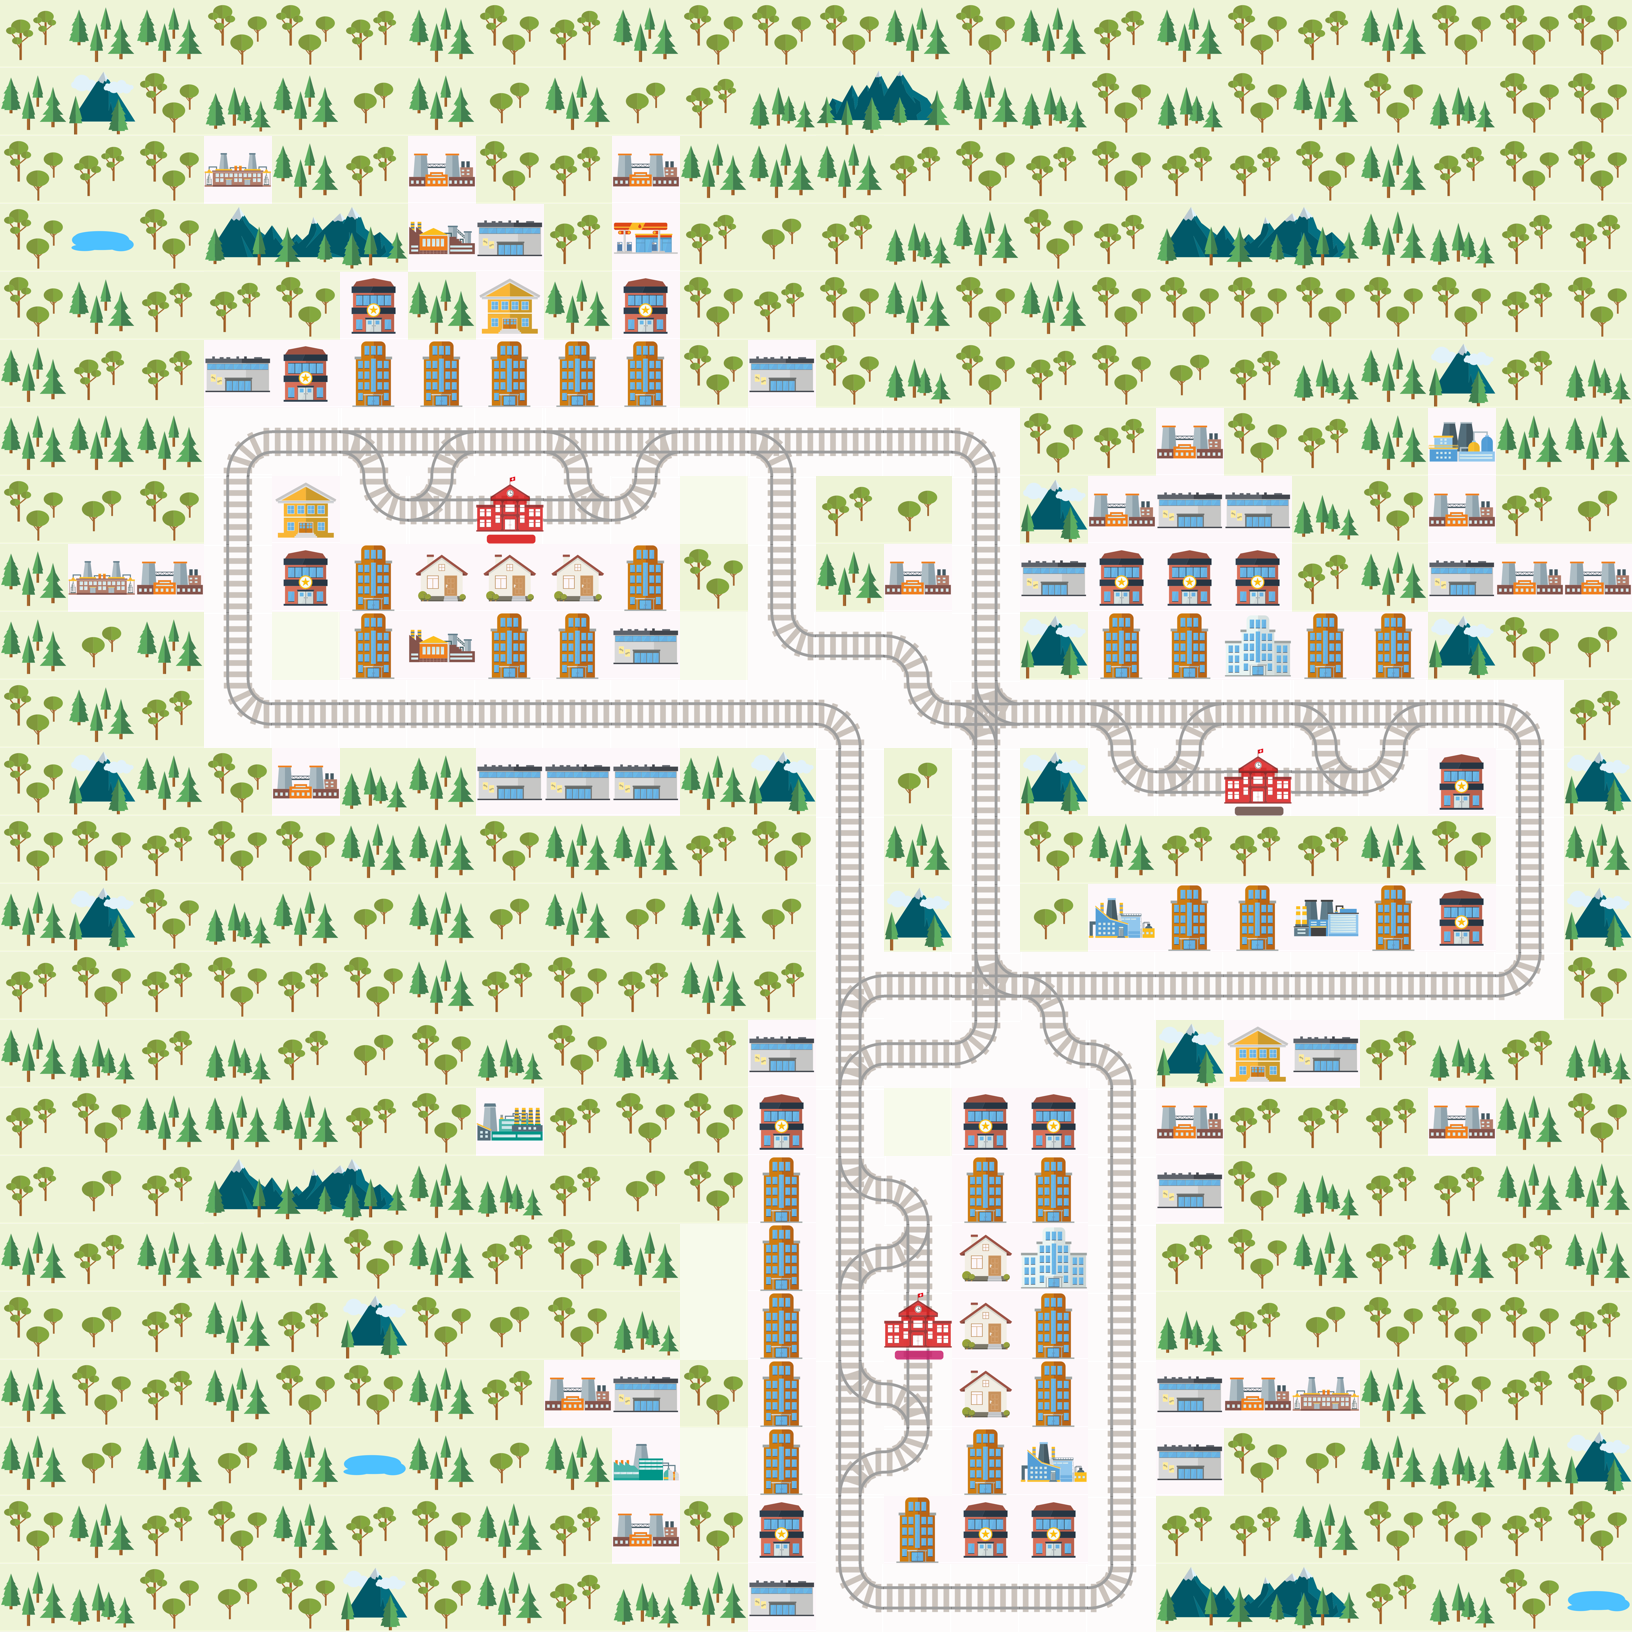
\includegraphics[width=0.48\textwidth]{dense/dense_0_1}
% 			\caption{Dense instance, using a 24x24 grid, where 20 trains must travel across 3 cities.}
% 			\label{dense_0_1}
% 		\end{subfigure}
% 	\hfill
% 		\begin{subfigure}{\textwidth}
% 			\centering
% 			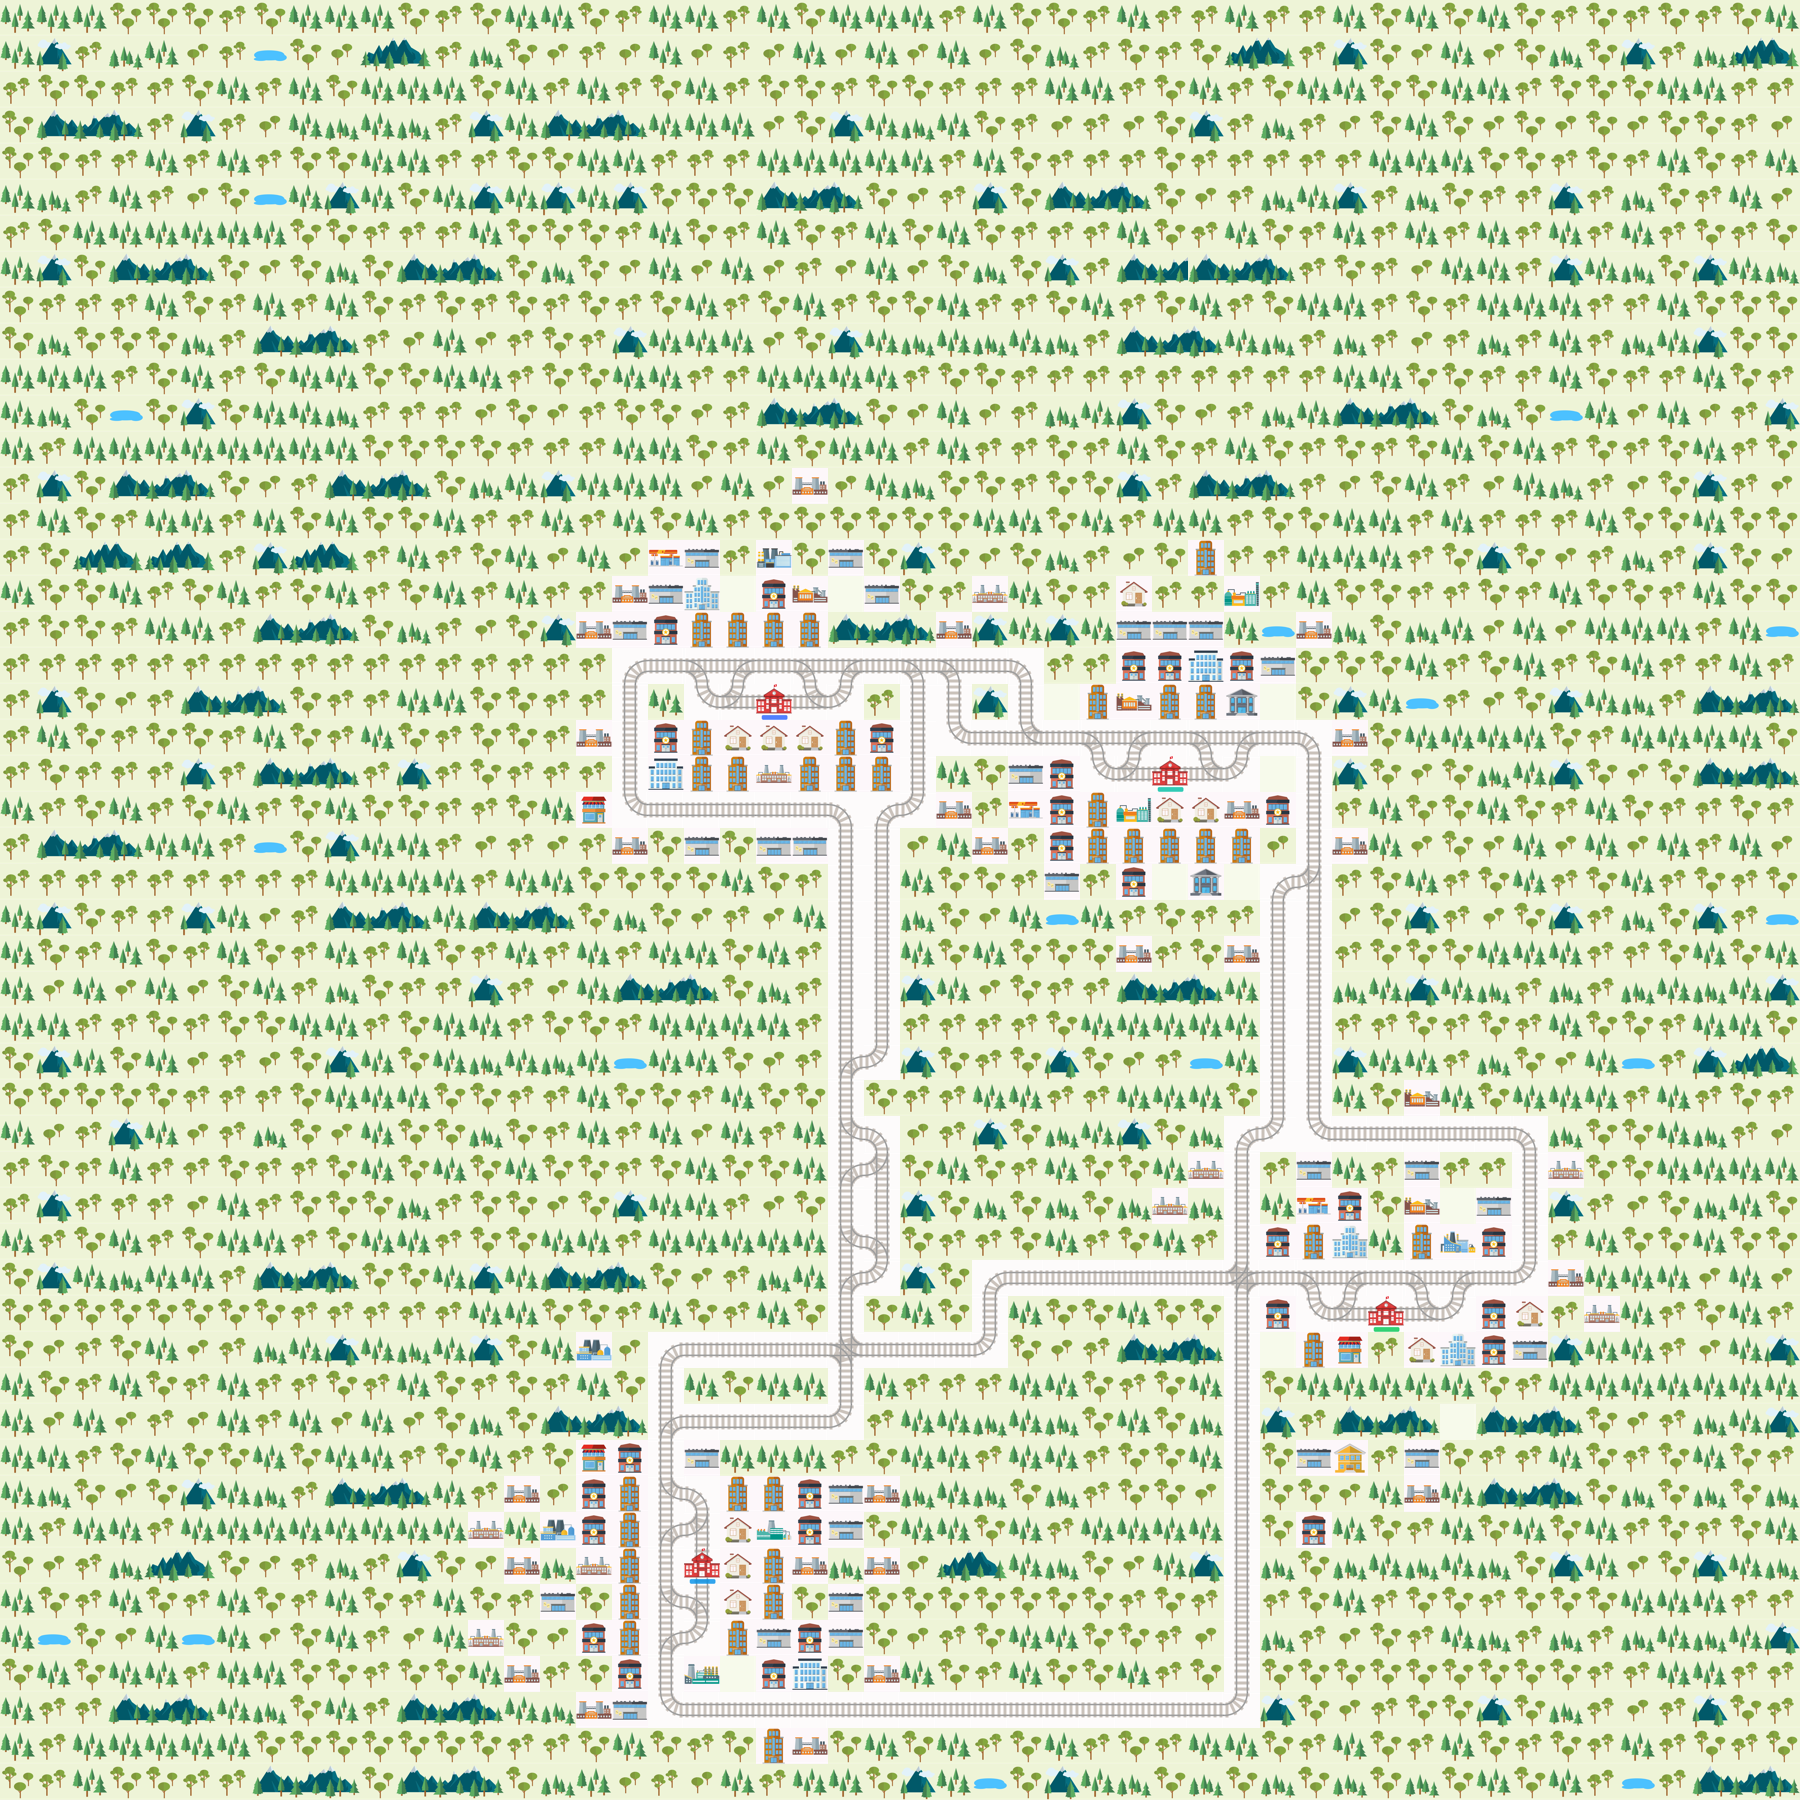
\includegraphics[width=\textwidth]{medium/medium_0_1}
% 			\caption{Medium instance, using a 50x50 grid, where 10 trains must travel across 5 cities.}
% 			\label{medium_0_1}
% 		\end{subfigure}
% 	\end{minipage}
% 	\hfill
% 	\begin{minipage}{.49\textwidth}
% 				\begin{subfigure}{\textwidth}
% 		\centering
% 		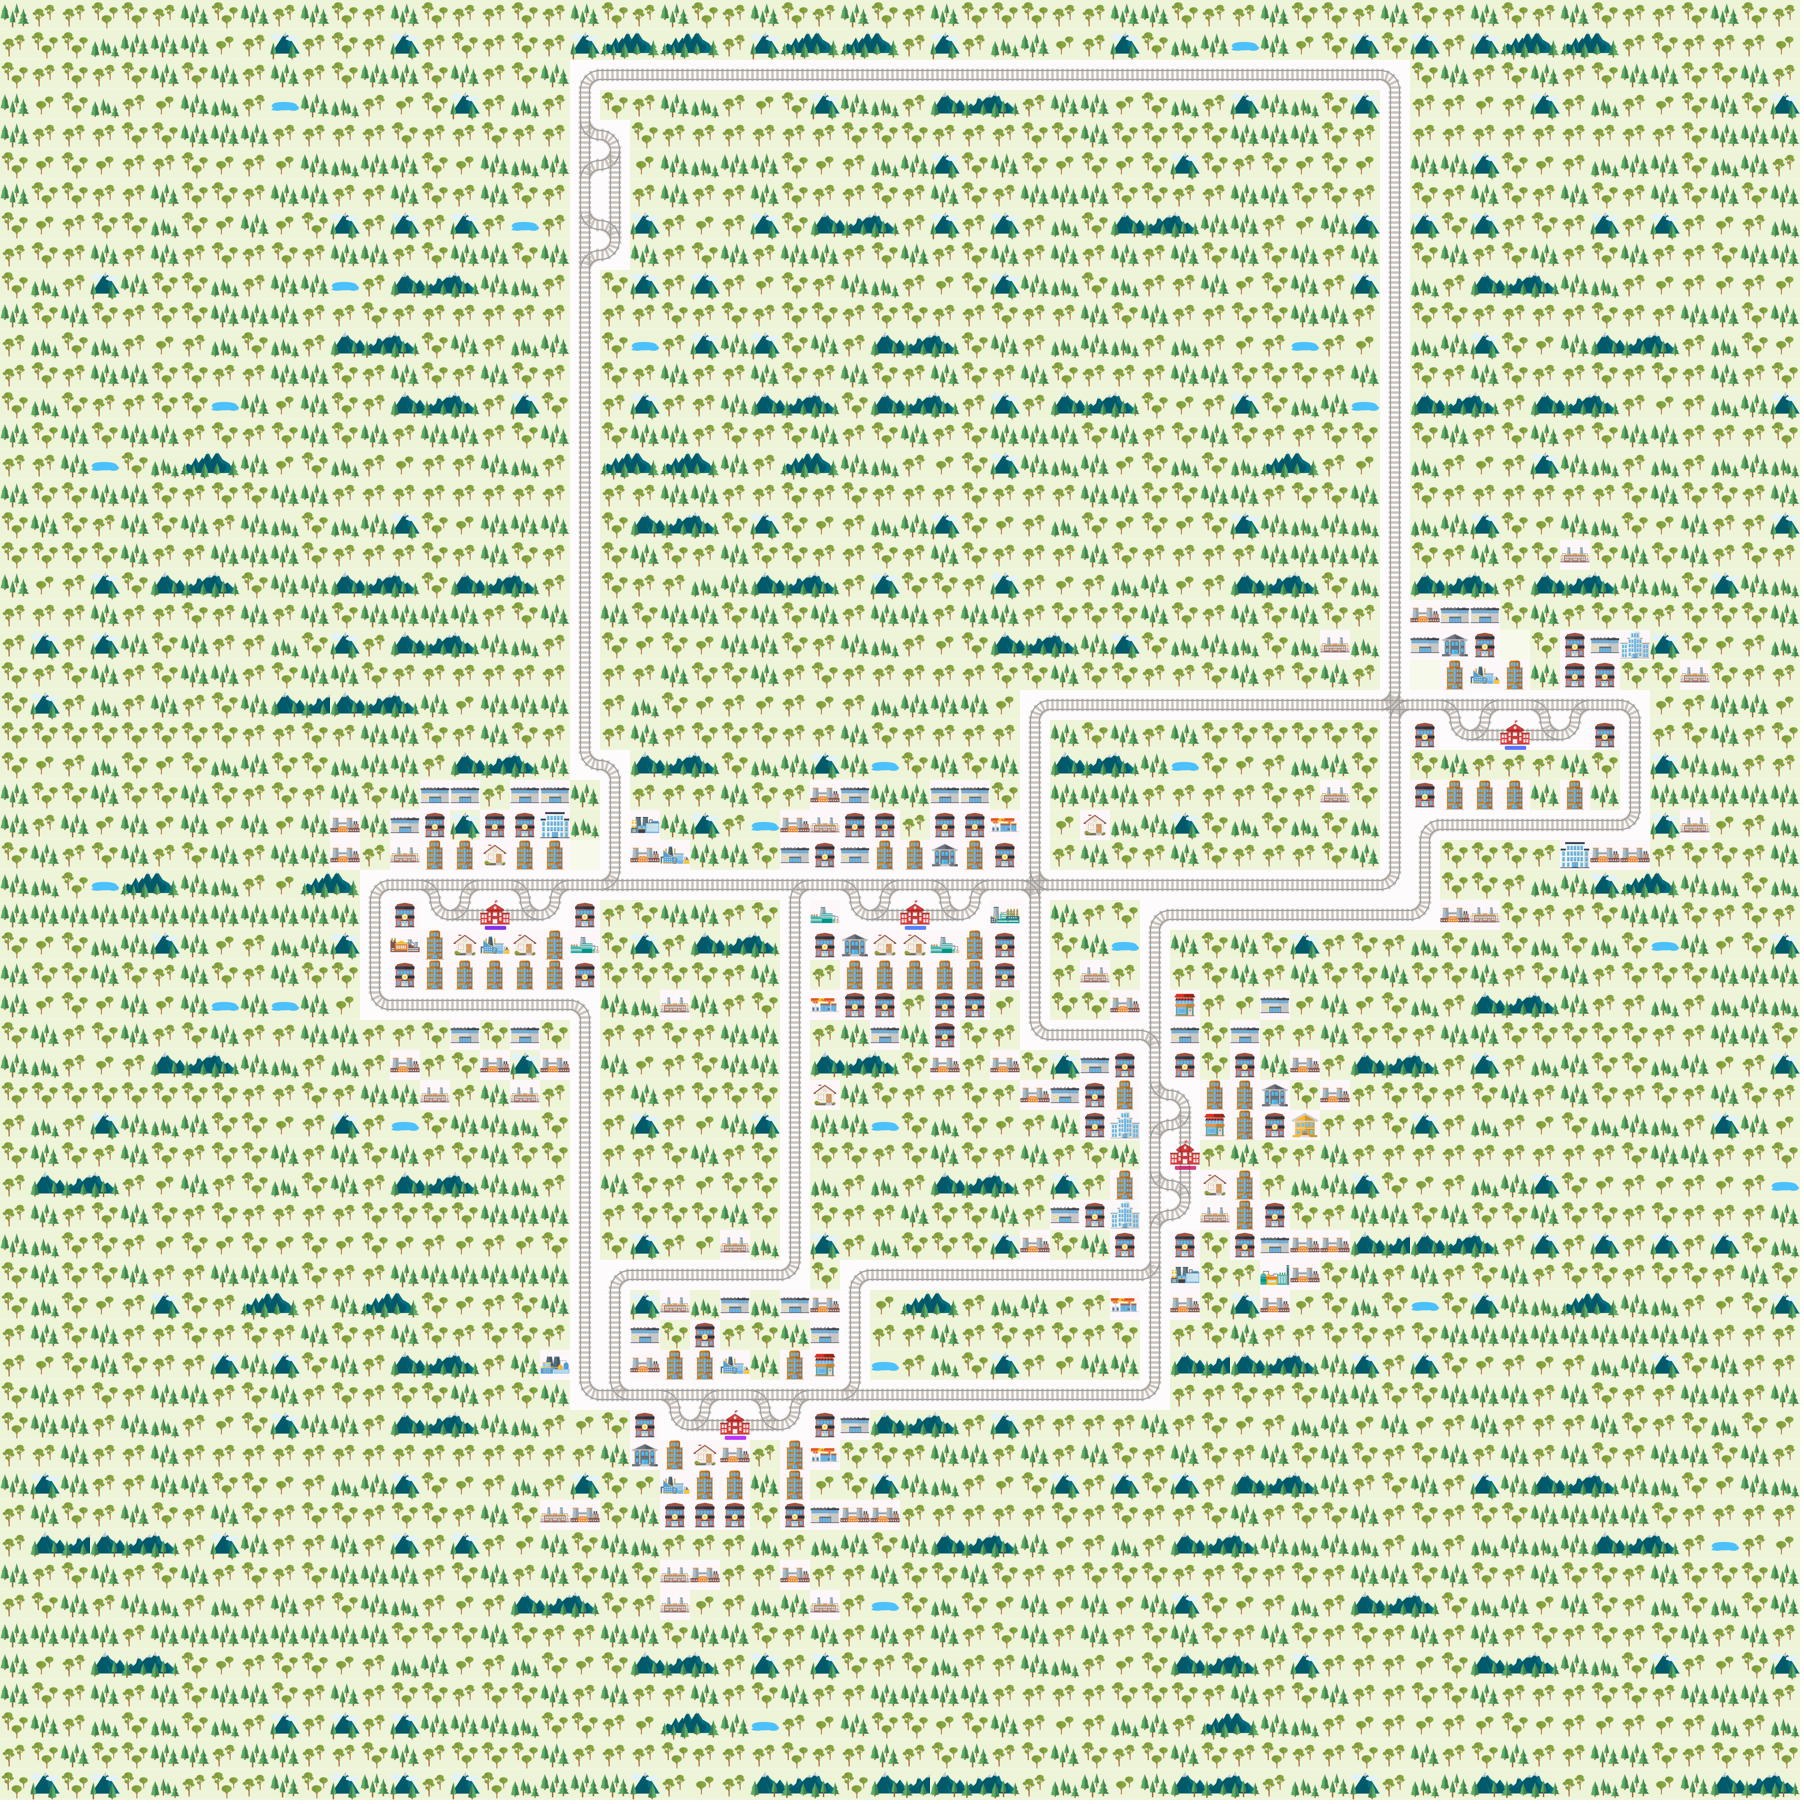
\includegraphics[width=\textwidth]{sparse/sparse_0_1}
% 		\caption{Sparse instance, using a 60x60 grid, where 6 trains must travel across 6 cities.}
% 		\label{sparse_0_1}
% 				\end{subfigure}
% 	\end{minipage}
% 	\caption{The 3 types of configurations used for our experimentation, put side-by-side in order to get an idea of the scale. The full list can be found at \cite{instance_folder}}
% 	\label{sparse_medium_dense}
% \end{figure}